% This must be in the first 5 lines to tell arXiv to use pdfLaTeX, which is strongly recommended.
% This must be in the first 5 lines to tell arXiv to use pdfLaTeX, which is strongly recommended.
\pdfoutput=1
% In particular, the hyperref package requires pdfLaTeX in order to break URLs across lines.

\documentclass[11pt]{article}

% Remove the "review" option to generate the final version.
\usepackage{naacl2021}

% Standard package includes
\usepackage{times}
\usepackage{latexsym}
\usepackage{caption}
\usepackage{subcaption}
\usepackage{graphicx}
\usepackage{float}
\usepackage{adjustbox}
\usepackage{graphicx}
\graphicspath{{./images/}}

% For proper rendering and hyphenation of words containing Latin characters (including in bib files)
\usepackage[T1]{fontenc}
% For Vietnamese characters
% \usepackage[T5]{fontenc}
% See https://www.latex-project.org/help/documentation/encguide.pdf for other character sets

% This assumes your files are encoded as UTF8
\usepackage[utf8]{inputenc}

% This is not strictly necessary, and may be commented out,
% but it will improve the layout of the manuscript,
% and will typically save some space.
\usepackage{microtype}

% If the title and author information does not fit in the area allocated, uncomment the following
%
%\setlength\titlebox{<dim>}
%
% and set <dim> to something 5cm or larger.

\title{Draft Technical Paper Working Title}

% Author information can be set in various styles:
% For several authors from the same institution:
% \author{Author 1 \and ... \and Author n \\
% Address line \\ ... \\ Address line}
% if the names do not fit well on one line use
% Author 1 \\ {\bf Author 2} \\ ... \\ {\bf Author n} \\
% For authors from different institutions:
% \author{Author 1 \\ Address line \\ ... \\ Address line
% \And ... \And
% Author n \\ Address line \\ ... \\ Address line}
% To start a seperate ``row'' of authors use \AND, as in
% \author{Author 1 \\ Address line \\ ... \\ Address line
% \AND
% Author 2 \\ Address line \\ ... \\ Address line \And
% Author 3 \\ Address line \\ ... \\ Address line}

\author{Alexander Mervar \\
 Indiana University \\
 \texttt{amervar@iu.edu} \\\And
 Aidan Rosberg \\
 Indiana University \\
 \texttt{arosberg@iu.edu}\\}

\begin{document}
\maketitle
\begin{abstract}
This paper presents a neural network method for predicting the average home cost of a given neighborhood. It builds from previous work in the area, and refines neural parameters and feature space to increase accuracy, and compares performance to linear regression and support vector models. It serves to demonstrate the usefulness of neural networks in the problem space.
\end{abstract}

\section{Introduction}

The Californian housing market is impacted not only by the features of a given house, but by the unique features of the surrounding landscape. This can mean that buyers do not only look at the qualities of a given home of interest, but also the qualities of the neighborhood the homes reside in that may be unique to the coastal state. While previous papers have focused on individual home costs and features, this paper seeks to demonstrate the efficacy of a neural network in predicting the average cost of homes in a neighborhood given the neighborhood’s proximity to the ocean, median income, population, and households, along with the average age and home features of the homes themselves.

Previous work examines housing market prediction with both pre-neural and neural methods. In pre-neural methods, regression models such as linear regression, support vector models (SVMs), Kohonen neural networks (KNNs), and random forest models have all been used to various degrees of success. Pow et al. (\citeyear{Pow2014}) demonstrated that KNNs and random forest models outperform baseline linear regression and SVMs, and speculate this is likely due to the ability to consider a higher vector space and draw connections beyond a linear plane. Later studies, such as Ćetković et al (\citeyear{Cetkovic2018}), examined the efficacy of neural network methods for market prediction, and found the results reasonable enough to continue refinement of parameters and further development of neural network methods in this field.

We seek to continue investigation into how best to harness the processing abilities of neural networks to solve the problem. This paper demonstrates that our neural network outperforms linear regression models, and shows how to refine the parameters of the neural network for best results.

\section{Dataset}

The dataset that we have selected is a collection of house data used in the second chapter of Aurélien Géron's book 'Hands-On Machine learning with Scikit-Learn and TensorFlow' (\citeyear{Geron2022}). The data contains information from the 1990 California census. Although this does not necessarily mean that our model can predict current housing prices, due to the volatility of the current economy and the nature of this project, it was decided that applying this methodology to current datasets would be outside the scope of this paper.

\subsection{Preprocessing Methods}

While the dataset we selected had already been preprocessed to an extent, we still took steps to ensure the efficacy of our models. The original dataset contained categorical values to express the distance of the given neighborhood from the coast. 
We applied one-hot encoding to extract these values to individual features. One-hot encoding was chosen to reduce bias introduced by other methods (Original encoding, Hashing). Another method employed to reduce bias was standardization. Because the ranges between the numerical values in the original data were high, we believed our neural model performance could be improved by scaling the values. We also applied mean imputation to estimate missing data.


\section{Methods}

\subsection{Linear Regression Model}

To test the validity of our neural network it was essential to create a linear regression to act as the baseline for comparison. By using Python packages pandas and statsmodels, we were able to fit the variables of the dataset to the "median\_house\_value" variable using a standard linear regression method. The coefficient table seen in \autoref{tab:lin-reg-table} was generated.

\subsubsection{Neural Network}

We created our artificial neural network with the Python package Tensorflow. Our model consists of three 64 node hidden layers a dropout layer to prevent over fitting, and we use RMSprop as our gradient decent optimizer. 
We experimented with multiple types of neural networks including convolutional and recurrent neural networks but our results had shown a conventional feed-forward artificial neural network provided the best results. 

\section{Results}
\subsection{Linear Regression Results}
Linear regression is a statistical method that is often used to model the relationship between a dependent variable and one or more independent variables. In the context of the housing market, linear regression could be used to predict the value of a house based on factors such as its location, size, age, and other characteristics.

One benefit of using a linear regression model for housing market predictions is that it is a simple and intuitive approach. Linear regression is based on the assumption that the relationship between the dependent and independent variables is linear, which means that it is easy to interpret and explain the results of the model. This can be particularly useful for real estate professionals who need to quickly and easily understand the factors that are influencing the value of a property.

Another benefit of using a linear regression model is that it is relatively easy to implement and run. Linear regression does not require complex algorithms or extensive data processing, which means that it can be run quickly and easily on most computers. This can be useful for real estate professionals who need to make fast, accurate predictions about the housing market.

However, there are also some downsides to using a linear regression model for housing market predictions. One major downside is that linear regression is only able to model linear relationships between the dependent and independent variables. This means that it is not able to accurately model complex, non-linear relationships that may exist in the data. In the context of the housing market, this could lead to inaccurate predictions, particularly in situations where the relationship between the dependent and independent variables is non-linear.

Another downside of using a linear regression model is that it is sensitive to outliers in the data. Outliers are data points that are significantly different from the rest of the data, and they can have a large impact on the results of a linear regression model. In the context of the housing market, this could mean that a few unusual properties could have a disproportionate influence on the predictions of the model, leading to inaccurate results.

In conclusion, the use of a linear regression model for housing market predictions has both benefits and downsides. It is a simple and intuitive approach that is easy to implement and run, but it is only able to model linear relationships and is sensitive to outliers in the data. These limitations should be considered when deciding whether to use a linear regression model for housing market predictions.

\subsection{Neural Network Results}

\begin{figure}[h]
\centering   
    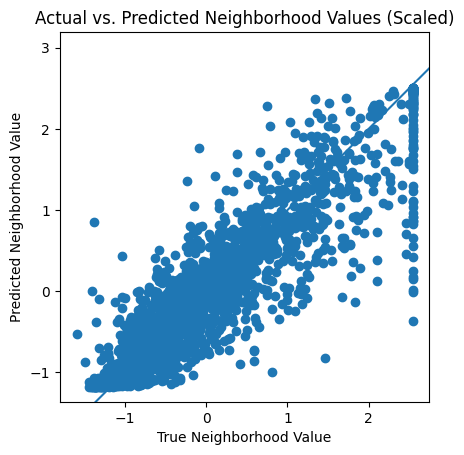
\includegraphics[scale=.5]{predictions}
    \caption{Actual vs. Predicted}
    \label{fig:pred}
\end{figure}

Our model had a mean squared error of $0.1837$ when we evaluated our testing data. As you can see from \autoref{fig:pred} our model struggled at predicting the value of neighborhoods with high value.  
\section{Discussion}
It is vital to compare the two methods and highlighting the key advantages of using a neural network over a linear regression.

One key advantage of using a neural network over a linear regression is its ability to model complex, non-linear relationships between variables. This is because a neural network is able to learn and identify patterns in the data that a linear regression cannot. This allows a neural network to make more accurate predictions, particularly in situations where the data is highly complex or has a lot of noise.

Another advantage of using a neural network is its ability to handle large amounts of data. Because a neural network is able to automatically identify patterns in the data, it is able to make predictions based on a large number of input variables, which can be difficult for a linear regression to handle. This allows a neural network to make more accurate predictions, even when dealing with large datasets.

Furthermore, a neural network is able to learn and improve over time. This is because a neural network is able to adjust its internal parameters based on the data it is given, allowing it to adapt to changing patterns in the data and make more accurate predictions. In contrast, a linear regression is unable to learn and improve over time, which can limit its accuracy in certain situations.


\section{Conclusion}
In conclusion, the use of a neural network over a linear regression offers several key advantages, which has been illustrated by the application here. It is able to model complex, non-linear relationships between variables, handle large amounts of data, and improve over time. These advantages make neural networks a valuable tool for making accurate predictions in the California housing market.


\appendix
\section{Appendix}
\begin{table*}[h]
    \centering
        \begin{tabular}{|l|l|l|l|l|l|l|} 
        \hline
        \textbf{variable} & \textbf{coef} & \textbf{std err} & \textbf{t} & \textbf{P\textgreater{}\textbar{}t\textbar{}} & \textbf{[0.025} & \textbf{0.975]} \\ 
        \hline
        longitude & -0.4594 & 0.018 & -26.092 & 0.000 & -0.494 & -0.425 \\ 
        \hline
        latitude & -0.4664 & 0.019 & -25.200 & 0.000 & -0.503 & -0.430 \\ 
        \hline
        housing\_median\_age & 0.1154 & 0.005 & 24.205 & 0.000 & 0.106 & 0.125 \\ 
        \hline
        total\_rooms & -0.0902 & 0.015 & -6.186 & 0.000 & -0.119 & -0.062 \\ 
        \hline
        total\_bedrooms & 0.2626 & 0.022 & 12.080 & 0.000 & 0.220 & 0.305 \\ 
        \hline
        population & -0.3853 & 0.010 & -36.896 & 0.000 & -0.406 & -0.365 \\ 
        \hline
        households & 0.2549 & 0.022 & 11.490 & 0.000 & 0.211 & 0.298 \\ 
        \hline
        median\_income & 0.6384 & 0.005 & 116.635 & 0.000 & 0.628 & 0.649 \\ 
        \hline
        ocean\_proximity\_1H OCEAN & 0.1072 & 0.007 & 14.790 & 0.000 & 0.093 & 0.121 \\ 
        \hline
        ocean\_proximity\_INLAND & -0.2370 & 0.011 & -21.579 & 0.000 & -0.259 & -0.216 \\ 
        \hline
        ocean\_proximity\_ISLAND & 1.4594 & 0.267 & 5.473 & 0.000 & 0.937 & 1.982 \\ 
        \hline
        ocean\_proximity\_NEAR BAY & 0.0752 & 0.015 & 5.048 & 0.000 & 0.046 & 0.104 \\ 
        \hline
        ocean\_proximity\_NEAR OCEAN & 0.1483 & 0.013 & 11.488 & 0.000 & 0.123 & 0.174 \\
        \hline
        \end{tabular}
\caption{Linear Regression Coefficient Table}
\label{tab:lin-reg-table}
\end{table*}

% Entries for the entire Anthology, followed by custom entries
\bibliography{custom.bib}
\bibliographystyle{acl_natbib}


\end{document}
